\documentclass[a4paper,11pt]{article}
\usepackage[T1]{fontenc}		% Seleção de códigos de fonte
\usepackage[utf8]{inputenc}		% Codificação do documento (conversão
\usepackage{indentfirst}		% Indenta o primeiro parágrafo de cada seção.
\usepackage{graphicx}			% Inclusão de gráficos
\usepackage{subcaption}				% enables the use of subfigures in floats
\usepackage[
%	a4paper,
left=2cm,
right=1.5cm,
bottom=1.5cm,
top = 2.5cm, 
foot=0.7cm]{geometry}
\usepackage{url}
\usepackage{setspace}
\usepackage{amsmath}
\usepackage{amsfonts}
\usepackage{fancyhdr}
\usepackage{multirow}
\usepackage{tabularx}
\usepackage{natbib}
\usepackage{import}
\usepackage[nottoc]{tocbibind} % insere as referências no sumário
\usepackage[brazil]{babel}
\usepackage{hyperref}
\usepackage{float}

\pagestyle{fancy}
\fancyhf{}
\lhead{DAS5151 - Instrumentação em Controle}
\rhead{Projeto Final}
\rfoot{\thepage}

\begin{document}
	\thispagestyle{empty}
\begin{center}
	
\includegraphics[height=2cm]{imagens/logoUFSCsimples.png} \\
	{\Large Universidade Federal de Santa Catarina -- UFSC} \\
	{\Large Centro Tecnológico -- CTC} \\
	{\Large Departamento de Automação e Sistemas -- DAS} \\
	\vspace{1cm}
	{\large Disciplina DAS 5151 - Instrumentação em Controle} \\
	\vfill
	\large{\textbf{Projeto Final} \\
	} 
	\vspace{1cm}
	% Integrantes: \\
    Bruno Machado Pacheco (16100865) \\
    \vfill
	Florianópolis, \today.
\end{center}

\clearpage

\tableofcontents

\clearpage

%%%%%%%%%%%%%%%%%%%%%%%%%%%%%%%%%%%%%%%%%%%%%%%%%%%%%%%%%

\section{Proposta do Projeto}

A proposta do projeto apresentado neste relatório é a instrumentação de um tanque cilíndrico de grande porte (2 m de altura e 1 m de diâmetro) para líquidos, com foco na indústria alimentícia. Entende-se o tanque como uma etapa de um processo maior da indústria alimentícia. No tanque, deseja-se controlar a temperatura de saída (para a próxima etapa) do líquido, que entra no tanque a temperatura ambiente. As condições de operação do líquido condizem com a faixa liquidez da água.

O tanque foi idealizado como possuindo isolamento nas paredes e na base, mas sendo aberto ao ambiente no topo. Imaginou-se que a injeção de líquido seria também pela superfície e que o líquido seria extraído pela base. Seria um requisito que a temperatura seja controlada de forma automática.

Um esquemático dos transdutores e atuadores propostos para o tanque pode ser visto na figura abaixo.

\begin{figure}[H]
    \centering
    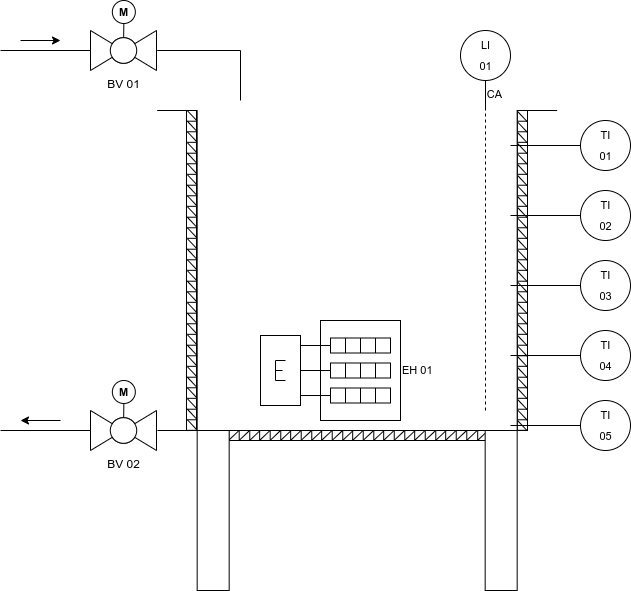
\includegraphics[width=0.8\textwidth]{imagens/tank.png}
    \caption{Diagrama dos transdutores e atuadores projetados para o tanque.}
    \label{fig:imagens-tank-png}
\end{figure}

Como pode-se ver, 5 transdutores de temperatura (TI 01 a 05) foram projetados para que seja possível o acompanhamento da temperatura ao longo do corpo do líquido, de forma a entender a distribuição de calor no mesmo. Além disso, um aquecedor (EH 01) interno foi projetado para que seja possível controlar a temperatura de saída do líquido. Para a vazão, duas válvulas (BV 01 e 02) e um transdutor de nível (LI 01) são esperados.


\newpage

\section{Planta}

As dinâmicas do líquido no interior do tanque foram simuladas no LabVIEW utilizando as ferramentas para equações diferenciais, em particular, para a equação do calor bidimensional para domínios retangulares. Como o tanque é cilíndrico, assumiu-se que simulando uma seção do tanque seria o suficiente para aproximar o comportamento da temperatura no interior do líquido frente aos pontos de medição almejados.

As condições de contorno foram utilizadas para simular as perdas e o aquecimento. Troca de calor nula nas paredes do tanque simulam o seu isolamento, enquanto uma injeção de calor constante (dentro de um passo de cálculo) nas paredes próximas ao aquecedor simulam a potência do aquecedor aquecendo o líquido. Para simular as perdas ao ambiente, a condução térmica entre o líquido e o ambiente externo (na distância entre a superfície e a abertura do tanque) foi calculada e definida como a perda de calor na superfície a cada passo de cálculo.

As variações volumétricas foram implementadas através de modificações no domínio de cálculo. Podemos entender o domínio de cálculo em uma situação computacional como uma matriz que representa as temperaturas nos pontos do líquido. Dessa forma, remoção do líquido perto da base foi emulada com a remoção das linhas da matriz mais próximas da base, enquanto adições de líquido foram feitas através de adições de linhas na matriz na região dos pontos da superfície do líquido.

Dessa forma, a cada passo de cálculo é necessário:
\begin{enumerate}
    \item Inicializar as equações e o domínio com a matriz de temperaturas resultante do passo anterior;
    \item Calcular as condições de contorno a partir dos valores do aquecedor e da temperatura ambiente;
    \item Resolver a equação do calor bidimensional para 1 passo de cálculo;
    \item Renderizar os resultados;
    \item Adicionar e remover linhas da matriz de acordo com a vazão de entrada e saída.
\end{enumerate}


\newpage

\section{Transdutores e Atuadores}

Os transdutores a atuadores foram escolhidos primeiramente visando atingir os objetivos propostos, mas também visando uma diversidade de circuitos de condicionamento de sinal necessários. Dessa forma, aproveitou-se do caráter virtual do projeto para que fossem experimentados diferentes abordagens.

Para o projeto dos circuitos de condicionamento, imaginou-se uma placa de aquisição e acionamento com limites de operação entre 0\,V e 5\,V, alta impedância e baixa potência de saída.

\subsection{Transdutores}

\subsubsection{Transdutores de temperatura}

\paragraph{Escolha dos componentes}\mbox{}

Para os transdutores de temperatura TI 01 a 05 foram escolhidos PT100, uma vez que possuem ampla utilização e possuem resposta suficiente para a aplicação, ou seja, sua sensibilidade na faixa de temperatura desejada é suficiente e não possui tempo de resposta impeditivo para um controle de temperatura.

De forma mais específica, o TRA-C61, da OPTITEMP foi selecionado uma vez que é um PT100 de Classe A e possui um tempo de resposta $t_{95\%} = 8,0$\,s. Além disso, possui já encapsulamento adequado para contato com alimentos. Ressalta-se que o ambiente do projeto é adequado também ao elemento sensor, uma vez que ele não sofrerá impactos no interior do tanque e também não haverá grande agitação.

\paragraph{Circuito de condicionamento}\mbox{}

Para condicionamento do sinal dos transdutores selecionados, utilizou-se uma medição a 4 fios e uma fonte de corrente. A queda de tensão sobre o PT100, então, alimenta um primeiro estágio de amplificação de diferenças para eliminar o \emph{offset} causado pela resistência de fio e um segundo estágio para eliminar o \emph{offset} padrão do PT100 e mapear a variação de 0\,ºC a 100\,ºC na faixa de 0\,V a 5\,V. Os resultados podem ser vistos na figura abaixo.

\begin{figure}[H]
    \centering
    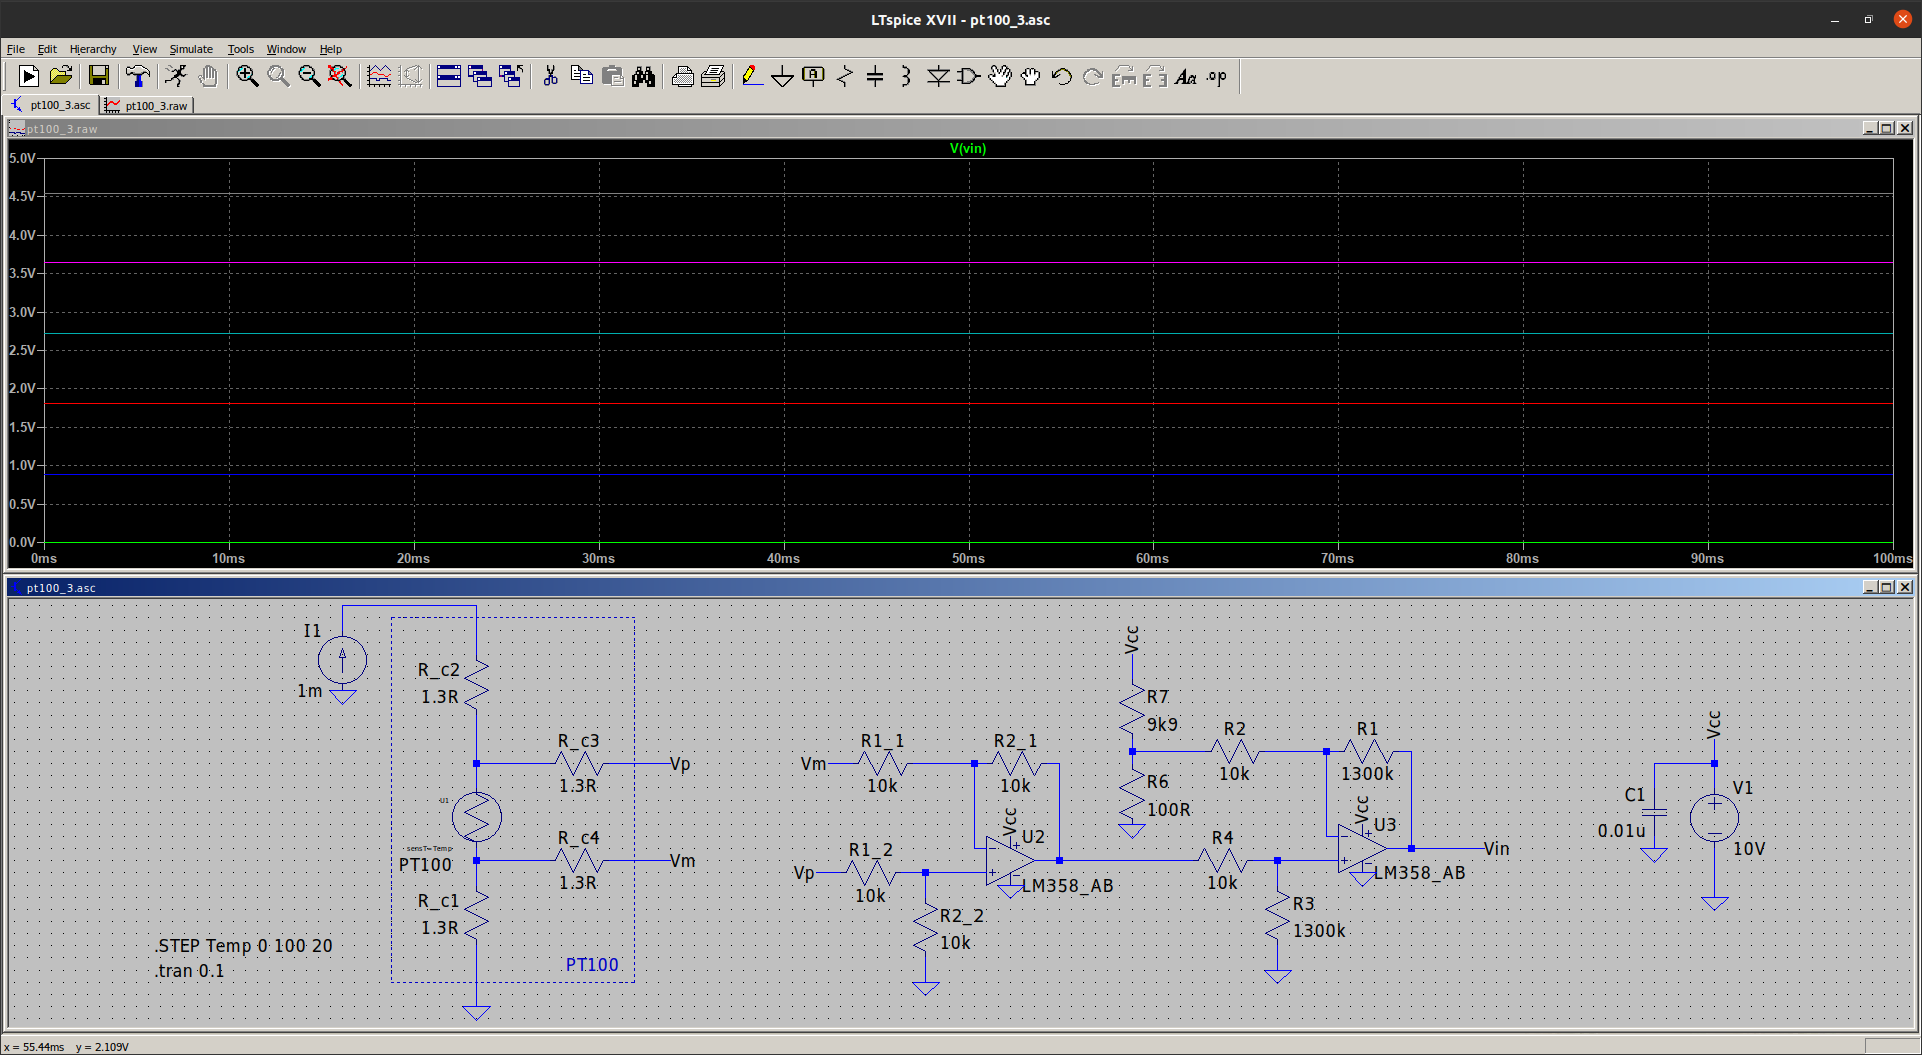
\includegraphics[width=0.8\textwidth]{imagens/temp_circ.png}
    \caption{Circuito de condicionamento de sinal do transdutor de temperatura e resultados da simulação. O nó \emph{Vin} simula a porta de leitura analógica do sistema de aquisição.}
    \label{fig:imagens-temp_circ-png}
\end{figure}

Como pode ser visto, os resultados ficaram cerca de 10\% abaixo do esperado. Essa variação também foi observada diretamente em cima do componente do transdutor, portanto, imagina-se que sejam causadas por parâmetros do próprio modelo SPICE do componente.

\paragraph{Simulação}\mbox{}

Para integrar o transdutor à simulação da planta, de forma a simular a implementação real da instrumentação, o transdutor foi simulado como um sistema de primeira ordem discreto seguido pelo tratamento do sinal, convertendo a grandeza física medida em um sinal na faixa de tensão que seria lida.

\subsubsection{Transdutores de Nível}

\paragraph{Escolha dos componentes}\mbox{}

As grandes limitações para a escolha de um transdutor de nível são a grande faixa de medição e a adequação a líquidos. Transdutores que se encaixam nessas restrições são transdutores potenciométricos de nível. Esses transdutores, muito utilizados em processos similares ao do escopo deste trabalho, comparam o potencial elétrico em uma haste metálica com a aquele da parede de um tanque ou de uma outra haste de referência. Dessa forma, eles fornecem rápida resposta, grande faixa de medição e suportam condições adversas.

O componente escolhido foi da série LSP-050.200.X.XXX, que possui uma haste de 2 metros e suporta variações de temperatura além daquelas do processo em questão. O transdutor tem tempo de resposta $t_{66\%} = 0,01$\,s, o que é muito além do necessário para a aplicação. Além disso, esse componente possui saída em corrente, em uma faixa de 4\,mA a 20\,mA, o que requer uma abordagem diferente para o condicionamento do sinal.

\paragraph{Circuito de condicionamento}\mbox{}

Para garantir a leitura adequada do sinal, um simples resistor foi utilizado para converter o sinal de corrente para tensão de forma que o sistema de aquisição pudesse realizar a leitura. A faixa de corrente do transdutor foi mapeada no intervalo de 1\,V a 5\,V. o \emph{offset} não foi compensado uma vez que o fabricante especifica que valores de corrente inferiores a 4\,mA indicam que o tanque está vazio, portanto, mapeadas em leituras a baixo de 1\,V. Além disso, não é um requisito a máxima resolução para o nível, não havendo perdas significativas para os resultados obtidos. O circuito projetado pode ser observado na figura abaixo, junto dos resultados da simulação.

\begin{figure}[H]
    \centering
    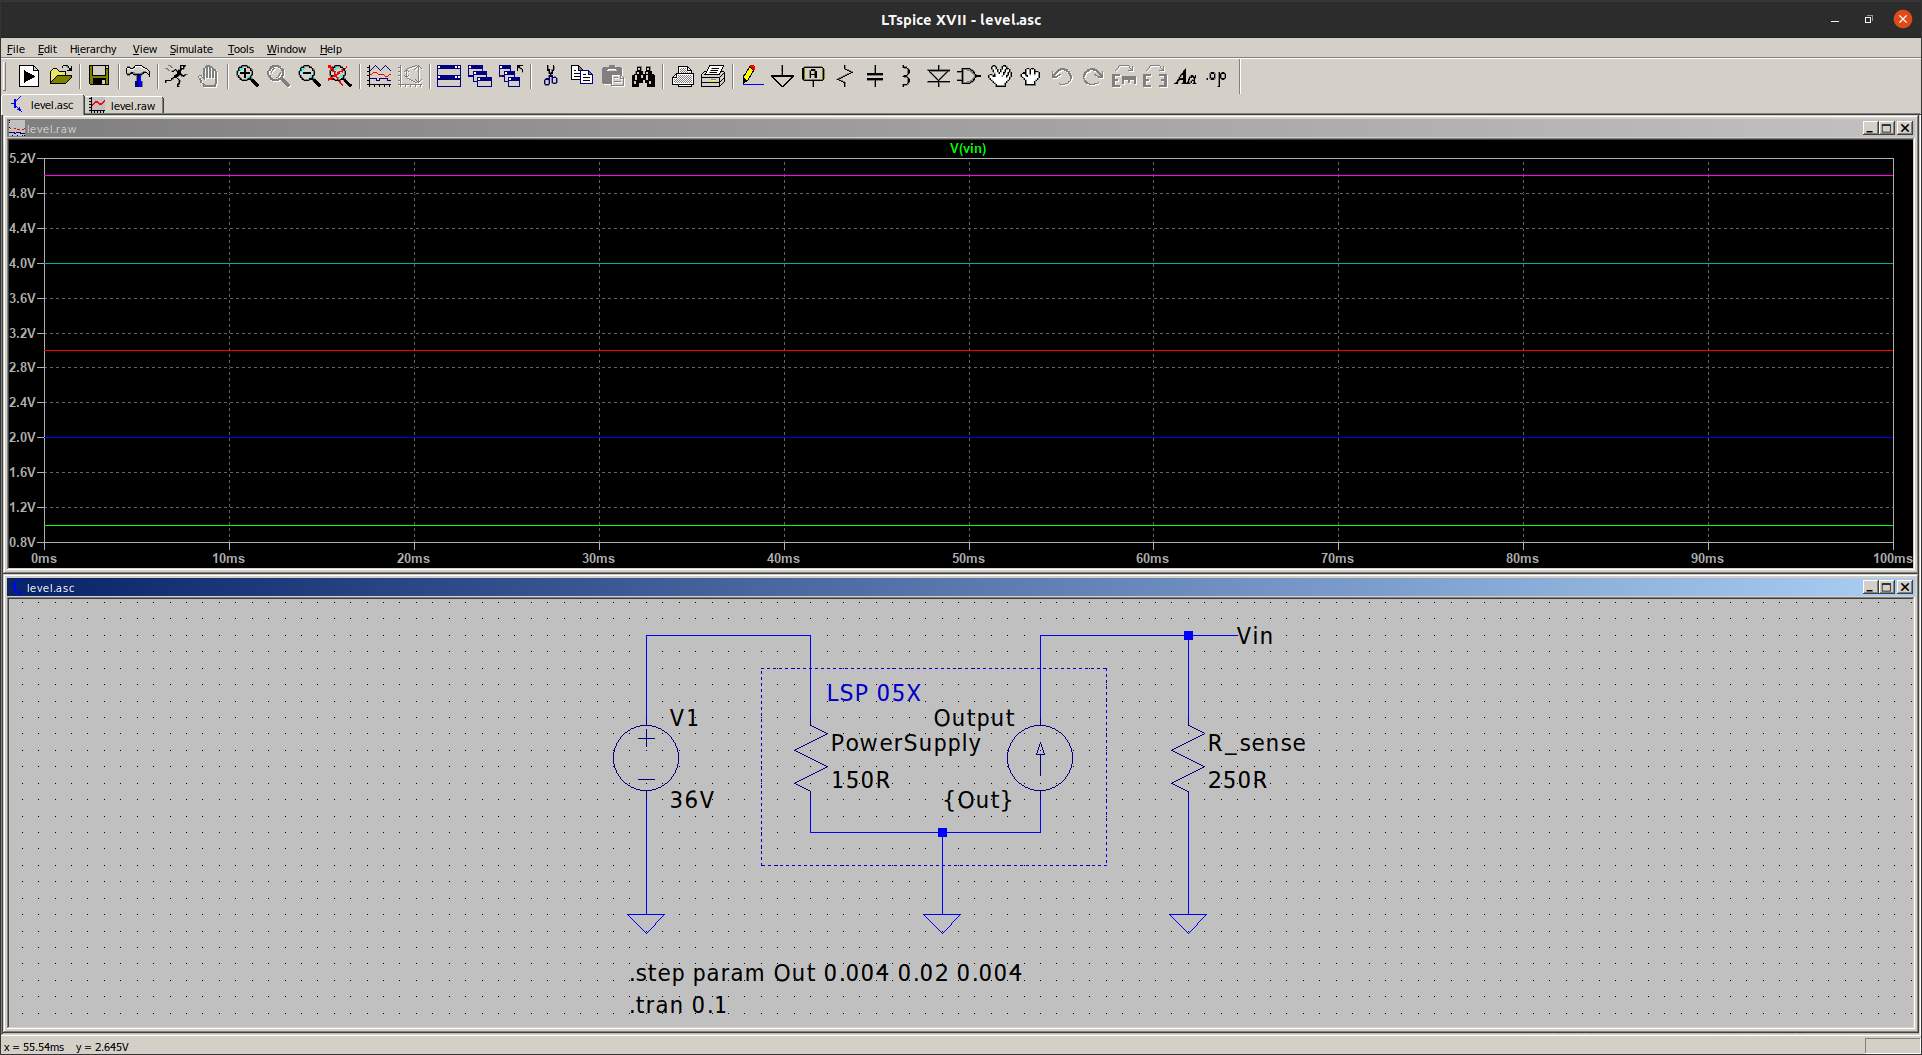
\includegraphics[width=0.8\textwidth]{imagens/level_circ.png}
    \caption{Circuito de condicionamento de sinal do transdutor de nível e resultados da simulação. O nó \emph{Vin} simula a porta de leitura analógica do sistema de aquisição.}
    \label{fig:imagens-level_circ-png}
\end{figure}

\paragraph{Simulação}\mbox{}

Ainda que bastante rápido frente os demais componentes do sistema, o transdutor de nível também foi simulado no LabVIEW como um sistema de primeira ordem seguido da conversão do nível de líquido para o sinal de tensão simulando o circuito de condicionamento.

\subsection{Atuadores}

\subsubsection{Aquecedor elétrico}

\paragraph{Escolha dos componentes}\mbox{}

A escolha de uma aquecedor elétrico adequado à aplicação passou pela necessidade do aquecimento de um grande volume de líquido, requerendo grande potência, e a simplicidade tanto do acionamento quando do modelo. Aquecedores de base, apesar de cogitados no início, não foram encontrados para tanques de grande porte. Soluções de aquecimento através de chamas também foram desconsideradas pela complexidade do acionamento e controle e por serem soluções sob medida, dificultando a obtenção dos parâmetros para modelagem.

Ao final, aquecedores submersíveis se mostraram alternativas bastante interessantes. São soluções altamente eficazes, uma vez que não há perda de calor para o ambiente, o que permite uma grande injeção de calor no líquido. O aquecedor TMT04014 foi tido como base, ainda que o modelo utilizado não tenha seguido fielmente as especificações do fabricante.

\paragraph{Circuito de condicionamento}\mbox{}

Como o aquecedor não possui sinais de controle, seu acionamento foi feito através da conexão com a rede elétrica. Para isso, um opto-DIAC foi utilizado para isolar a placa de controle da rede e um TRIAC em cascata foi utilizado para suportar a corrente do aquecedor e a tensão da rede. Os resultados podem ser observados na figura abaixo.

\begin{figure}[H]
    \centering
    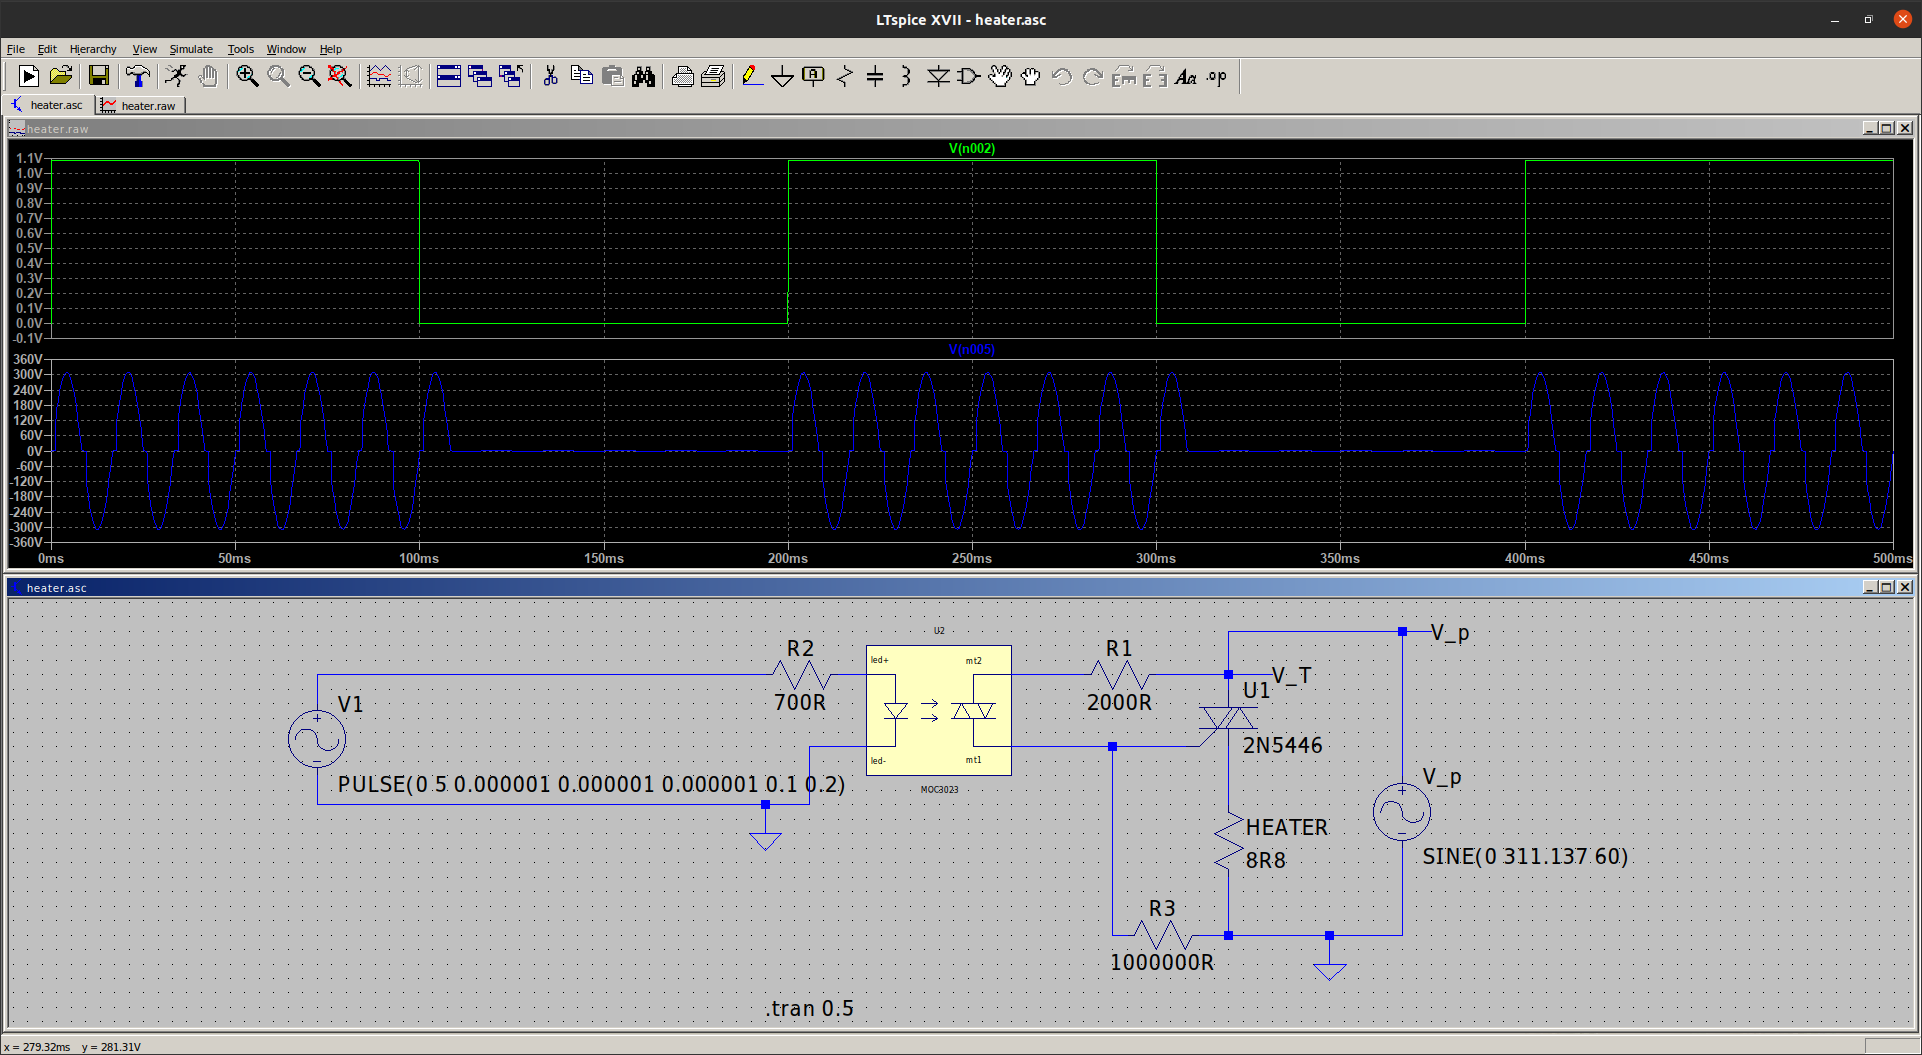
\includegraphics[width=0.8\textwidth]{imagens/heater_circ.png}
    \caption{Circuito de acionamento do aquecedor elétrico e resultados da simulação. A fonte \emph{V1} simula o sinal de saída da placa de controle, enquanto a fonte \emph{V\_p} simula a tensão da rede elétrica.}
    \label{fig:imagens-heater_circ-png}
\end{figure}

\paragraph{Simulação}\mbox{}

Infelizmente, a fabricante não disponibiliza o tempo de resposta do aquecedor. Dessa forma, assumiu-se que a potência consumida é imediatamente injetada no sistema, ou seja, desprezou-se o tempo de resposta. Ainda mais, a troca de calor utilizada no modelo do tanque como base para a simulação foi uma estimativa da gerada pelo aquecedor, uma vez que a modelagem de trocadores de calor foge do escopo deste trabalho. Dessa forma, o modelo no LabVIEW foi uma simples conversão do sinal binário do acionamento digital para o calor gerado na base do modelo do tanque.

\subsubsection{Válvulas}

\paragraph{Escolha dos componentes}\mbox{}

Para o controle da vazão de entrada e de saída de forma a regular o nível no tanque é de interesse utilizar válvulas que tenham uma resposta linear ao acionamento. Felizmente, os requisitos de pressão suportada são baixos, uma vez que não há especificação para a válvula de vazão de entrada e a vazão de saída está submetida somente à pressão hidrostática da coluna de água do tanque.

Para maximizar a vazão, a válvula R2050-40-S4 da fabricante BELIMO foi escolhida. Além de ser uma válvula esférica (relação linear entre vazão e ângulo de abertura), ela possui o maior coeficiente de vazão (kvs de 40\,m$^3$/h) dessa linha. Além disso, ela também suporta a faixa de temperatura do processo. Para seu acionamento, o atuador rotacional LR24A-SR da mesma fabricante foi selecionado. Além de ser recomendado pela fabricante, o que dá garantia de funcionamento, ele possui atuação linear na faixa de 2 a 10 V, mantendo a válvula fechada em tensões inferiores à faixa. Infelizmente, esse atuador possui um tempo de resposta de 90\,s/\,90º.

\paragraph{Circuito de condicionamento}\mbox{}

O circuito para acionamento desse conjunto pode ser visto na figura abaixo, junto dos resultados da simulação. Como não há requisito de ajuste fino da vazão, foi implementado um simples amplificador, deixando a cargo do controle regular a válvula dentro da faixa de 1 a 5 V, mantendo-a fechada abaixo dessa faixa.

\begin{figure}[H]
    \centering
    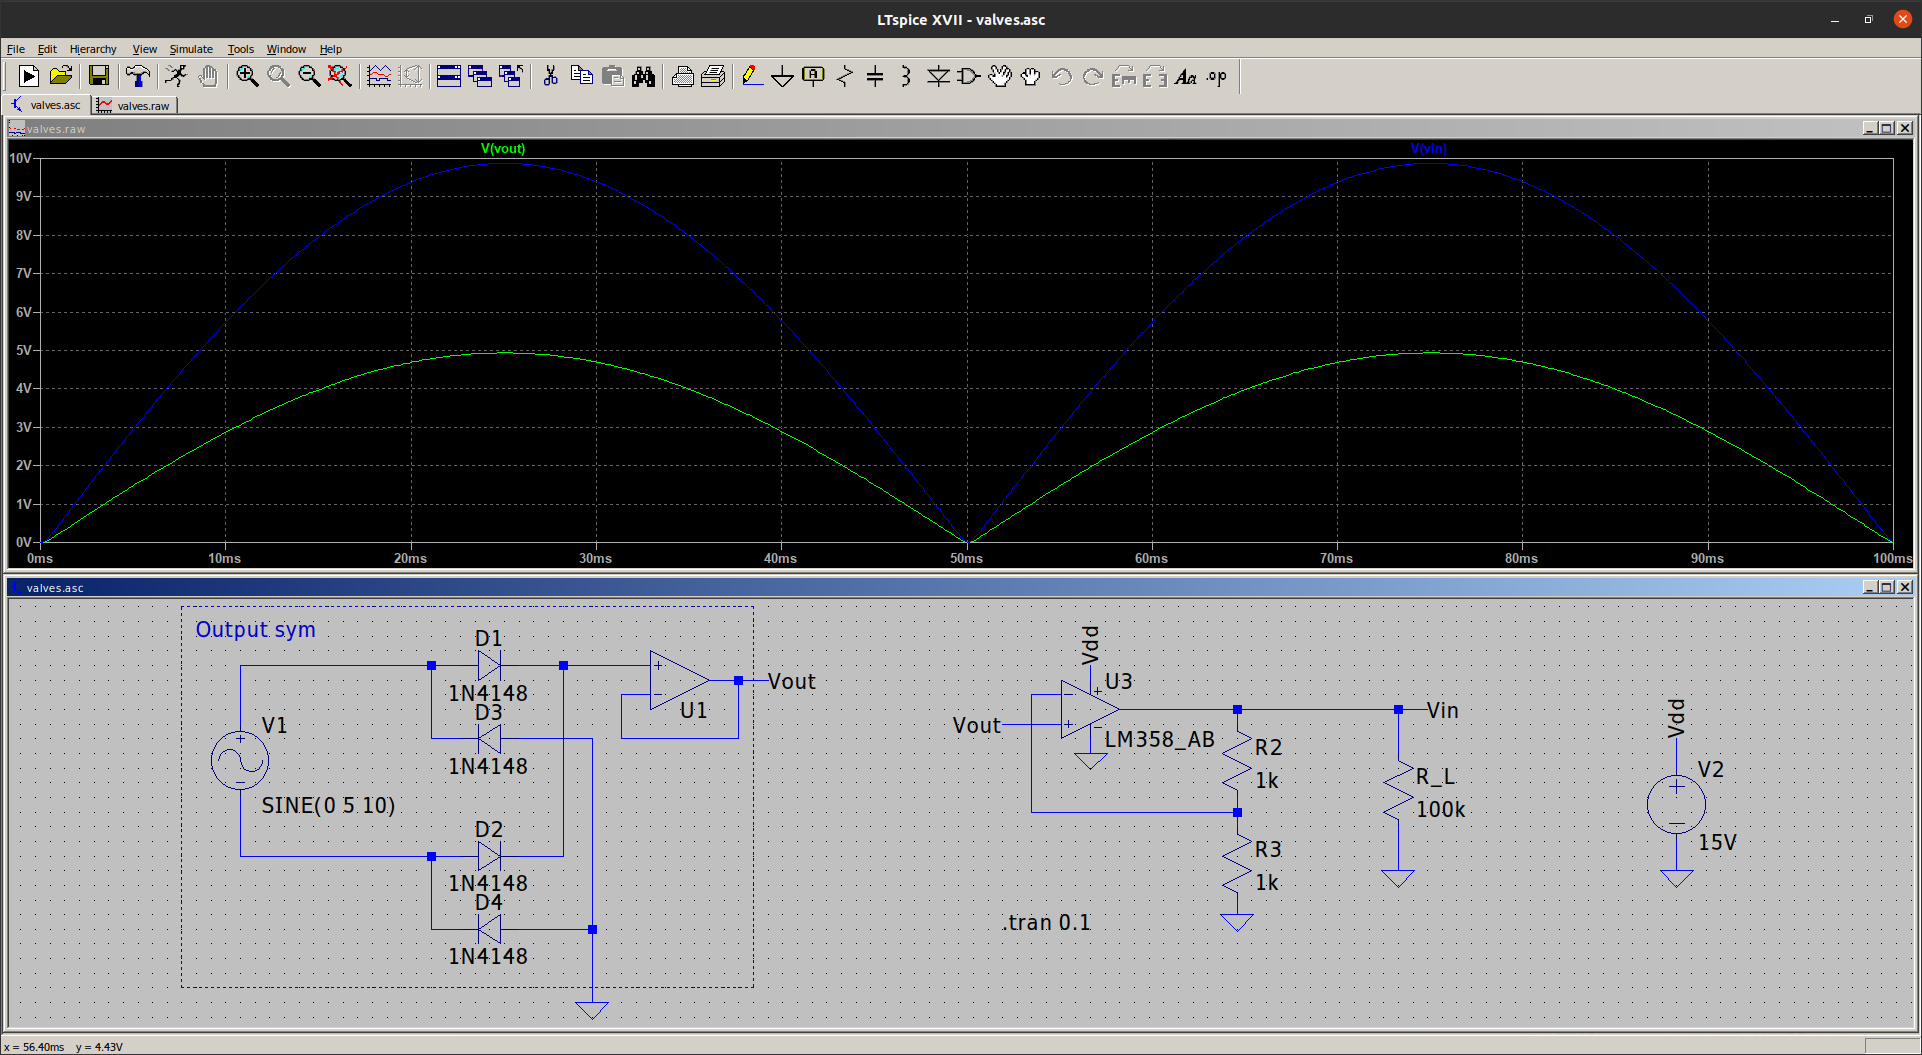
\includegraphics[width=0.8\textwidth]{imagens/valves_circ.png}
    \caption{Circuito de acionamento dos conjuntos das válvulas e resultados da simulação. A saída \emph{Vout} foi tal que simule uma varredura da saída analógica da placa de acionamento. O nó \emph{Vin} simula a entrada do atuador junto da impedância interna \emph{R\_L}.}
    \label{fig:imagens-valves_circ-png}
\end{figure}

\paragraph{Simulação}\mbox{}

Supôs-se que a limitação de velocidade da válvula é relativa à velocidade rotacional do motor, ou seja, o motor opera a 1º\,/\,s. Dessa forma, o tempo de resposta foi simulado com pequenos incrementos do valor do ângulo de abertura da válvula até que se atingisse o valor desejado. Além, é claro, da simulação do condicionamento do sinal.


\newpage

\section{Protótipo}

Para simular o sistema de forma integrada, foram unidas as simulações da planta (como descrita na seção 2) e dos transdutores e atuadores (como descritas na seção 3). Dessa forma, foi adicionada a lógica de controle e processamento dos sinais, de forma a simular um sistema supervisório e de controle da planta.

De forma a manter as simulações modulares e independentes, ou seja, mais fidedignas, foram simulados 3 laços de repetição em paralelo. O primeiro simula o tanque e suas grandezas físicas. O segundo, os transdutores e atuadores bem como seus circuitos de condicionamento. Finalmente, o terceiro implementa o tratamento de sinal e a lógica de controle. Todos esses componentes se encontram bem documentados nos arquivos do projeto do LabVIEW.

Para a comunicação entre os laços foram utilizados controladores e indicadores invisíveis, evitando o uso de variáveis ou intertravamento entre os laços. Dessa forma, o laço que simula a planta se comunica com os indicadores/controladores que representam as grandezas físicas de interesse, e.g., a temperatura no elemento sensor dos transdutores de temperatura, a potência fornecida pelo aquecedor elétrico. Já o laço que simula os transdutores e atuadores e seus circuitos faz a ponte entre os indicadores/controladores recém mencionados e aqueles que representam as tensões lidas fornecidas pela placa de controle, e.g., tensão lida no TI 01, tensão escrita na porta ligada ao circuito do BV 01. Finalmente, o laço de tratamento de sinal e controle lida com os valores tangíveis à placa no que se relaciona com a interação com o usuário e a lei de controle.

O resultado da união das 3 estruturas é mostrado no painel frontal da principal VI do projeto, como visível na figura abaixo. O controle da temperatura ambiente, apesar de fora do alcance do usuário na aplicação real, foi mantido para estudo dos efeitos desse ruído. Também para facilitar a compreensão do modelo, o gráfico da temperatura ao longo do líquido foi mantido.

\begin{figure}[H]
    \centering
    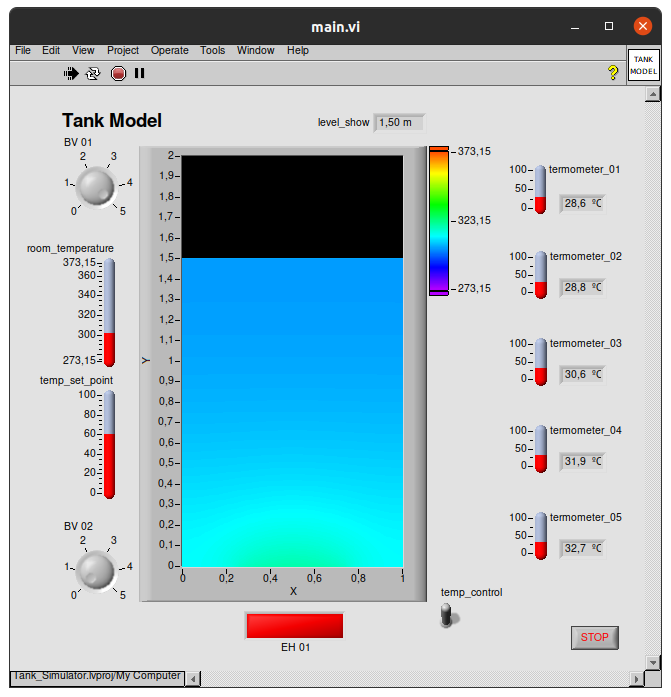
\includegraphics[width=0.6\textwidth]{imagens/main_frontpanel.png}
    \caption{Painel frontal da VI principal do projeto.}
    \label{fig:imagens-main_frontpanel-png}
\end{figure}


\newpage

\section{Desafios}

Ainda que devido à modalidade remota o projeto não envolva um protótipo real, vários desafios foram encontrados principalmente na tentativa de fazer simulações fidedignas. O primeiro desafio encontrado, em ordem cronológica das implementações, foi quanto à estabilidade da simulação do líquido no tanque. As variações do domínio das equações decorrentes das vazões de entrada e saída facilmente ocasionavam instabilidades nos resultados ao longo do tempo. Muitas vezes, isso decorria de erros de arredondamento que se acumulavam ao longo do tempo, fazendo com que o nível da água esperado e o tamanho da matriz que armazena os pontos no interior do líquido divergissem. A solução encontrada foi limitar a vazão máxima (a 0,5\,m$^3$/s, um valor bastante alto) e realizar somente incrementos proporcionais à resolução da matriz do domínio, passando ao passo seguinte as variações de volume restantes.

Além disso, a definição do modelo da planta antes da escolha dos componentes (devido à ordem das entregas) limitou as escolhas a soluções não necessariamente ideais. Um exemplo é o aquecedor elétrico, que esperava-se utilizar um sistema de aquecimento por contato com a base do tanque, mas soluções satisfatórias (grande porte, fornecimento de potência suficiente, disponibilidade de dados) dessa forma não foram encontradas, resultando na escolha de um sistema de aquecimento não muito adequado à simulação.

Já no âmbito da integração dos componentes da simulação, a pequena vazão das válvulas acabou limitando o seu potencial como fontes de ruído para a malha de controle. A falta de experiência no dimensionamento desse tipo de componente hidráulico acabou limitando a escolha a válvulas de baixo coeficiente de vazão, de forma que a pequena diferença de pressão estipulada não fosse suficiente para gerar um impacto significativo na condução térmica.

Finalmente, a ausência de suporte de muitas das ferramentas para o sistema operacional Linux tornou necessária a simulação dos circuitos de condicionamento utilizando um software especifico para isso (LTSpice) que não consegue se comunicar com o software desenvolvido em LabVIEW para monitoramento e controle. Isso gerou um esforço adicional para modelar o desempenho dos circuitos no LabVIEW, de forma que a malha de controle pudesse ser completada.

\section{Próximos Passos}

É evidente que o presente trabalho possui muita margem para melhoria. Ainda assim, o foco desta seção será em potenciais aprimoramentos no que tange o escopo da disciplina. Dessa forma, por exemplo, modificações na simulação do líquido no interior do tanque ou no processo em questão não serão abordadas. Além disso, as melhorias propostas são sempre tendo em vista a experiência adquirida com o presente trabalho, e não necessariamente o desempenho do processo imaginado no qual se enquadra o sistema simulado.

Dito isso, uma escolha de componentes mais adequados a aplicação pode ser feita. Válvulas que permitam maior vazão ou o uso de uma bomba para aumentar a diferença de pressão na válvula de saída permitira um controle mais dinâmico do nível. Um aquecedor com controle do calor gerado permitiria a implementação de um controlador PI, por exemplo, dando muito mais precisão à temperatura do líquido de interesse.

Melhorias nos modelos dos transdutores e atuadores seriam de grande benefício para que os resultados se tornem mais confiáveis. Exemplos seriam um modelo do aquecedor elétrico que considere seu tempo de resposta e um modelo do transdutor de nível que considere os efeitos da temperatura do líquido. Além disso, seria interessante simular ruídos de forma a tornar válida a implementação de filtros nos sinais mais críticos, analisando o impacto dos ruídos no desempenho do controlador. Finalmente, seria também interessante simular, através de um componente aleatório, os erros dos transdutores de acordo com as margens fornecidas pelos fornecedores.


\newpage

\end{document}
